\documentclass[10pt,a4paper]{article}
\usepackage{fullpage}
\usepackage{fancyvrb}
\usepackage[latin1]{inputenc}
\usepackage{amsmath}
\usepackage{amsfonts}
\usepackage{amssymb}
\usepackage{framed}
\usepackage{pstricks}    %for embedding pspicture.
\usepackage{graphicx}
\usepackage{hyperref}
% (1) choose a font that is available as T1
% for example:
\usepackage{lmodern}

% (2) specify encoding
\usepackage[T1]{fontenc}

% (3) load symbol definitions
\usepackage{textcomp}

% needed for small caption fonts
\usepackage[skip=2pt]{caption}

\DeclareCaptionFormat{myformat}{\fontsize{8}{9}\selectfont#1#2#3}
\captionsetup{format=myformat}
\bibliographystyle{plain}
\author{Adam Gibson}
\begin{document}

\title{An investigation into Confidential Transactions.}
\maketitle

\section{Introduction}

\vskip 0.1 in \noindent \underline{What this document is not}:
\begin{itemize}
\item It is \textbf{not} an explanation of sidechains.
\item It is \textbf{not} even a complete explanation of Confidential Transactions. It is already very long, but misses a few things like special cases involving unblinded inputs/outputs.
\item It is \textbf{not} guaranteed to be accurate, although obviously every effort has been made. You do not have permission to put money on the line based on what is written here (although I do give full permission for you to lose all your testnet coins).
\end{itemize}

\vskip 0.1 in \noindent \underline{What this document is}:
\vskip 0.1 in \noindent This serves as an amplification to \cite{ct_wu}. Both that document and this are describing the operation of the code in Elements Alpha project which is available here: \url{https://github.com/ElementsProject/elements/tree/alpha/src}. Note that it is already possible to build and run this code, though it is (of course!) in alpha and not production ready (also, the implementation uses testnet rather than Bitcoin mainnet).

\vskip 0.1 in \noindent If you want to understand in detail how CT (I will use this abbreviation for `Confidential Transactions') works, this document may be useful. How useful it is to you personally will depend on your technical level.
\vskip 0.1 in \noindent If you are a complete beginner to Bitcoin, this is probably not for you. If you are an expert cryptographer, then the introductory sections are definitely not for you, as they include wordy descriptions of basic constructs (commitments for example). You would probably be better off going straight from \cite{ct_wu} to the code. The section at the end might serve as a useful starting point on the mechanics of Confidential Transactions.


\subsection{Prerequisites}

I have endeavoured to make this description understandable to a relative novice in the cryptographic concepts, but of necessity some basic knowledge has to be assumed. Detailed understanding of algorithms aren't assumed (you \textit{don't} have to know: how to construct a hash function, how to add points on an elliptic curve, any details about what is required to make these constructs fully cryptographically secure). A passing familiarity with these concepts is helpful, though:

\begin{itemize}
\item Modular arithmetic. Not theorems about it, but simply how adding and subtracting works in mod $N$.
\item What makes cryptographic hashes (here, SHA256, although that isn't important) useful.
\item Elliptic curve arithmetic basics (what you can and can't do with elliptic curve points, not \textit{how} you do it).
\item The main idea of elliptic curve asymmetric cryptography: specifically, public and private keys and their relationship.
\item The basic structure of a Bitcoin transaction (but \textbf{not} the lower level detail, e.g. Bitcoin Script).
\end{itemize}

\vskip 0.1 in \noindent I would hazard a guess that a person who's got as far as opening this document is not very likely to find the mathematics unintelligible. I would caution two things: (1) this a complicated structure, and takes time to digest, and (2) if you have never seen or understood simple examples involving adding elliptic curve points, then refer to one of the several primers on the net that exist for beginners in elliptic curve cryptography.

\vskip 0.1 in \noindent A note about notation: when doing elliptic curve arithmetic, it's traditional to use lower case letters for ordinary numbers (integers) and upper case letters for curve points. Hence, in $xG + aH$, $x$ and $a$ are ordinary numbers and $G$ and $H$ are curve points.

\subsection{Goals}

Starting in a moment, things get technical very fast. It's important to understand where we're going. The idea of having transactions be private in a digital cash context is very old. David Chaum, in particular, blazed a trail in designing a kind of money where the amount could be hidden (blinded) while it was still ensured that money was not being stolen or created from nothing \cite{chaum_bs}. This idea was initially applied to the following context: you want a bank to be the issuer of digital cash, but you want the users of the cash to be able to transact amounts that are kept private from the bank and any other observers. What will be described in this document, CT, is an attempt to create the same effect but in the much more radical context of a decentralised network, i.e. Bitcoin or more specifically a sidechain using Bitcoin.

\vskip 0.1 in \noindent The core idea behind how to achieve this is closely connected to the idea of ``homomorphic encryption''. Suppose you have a bunch of data (\$100, -\$4, \$231) and you want to give that data to someone else to compute something - like the total - but you don't want that person to know what the amounts are - either the inputs, or the output (the result). Cryptography can do this for you, and it's (in certain contexts) called ``homomorphic'' (preserving structure being the crude meaning). Some of the rules of arithmetic that apply to the plain amounts also apply to the encrypted amounts, but the encrypted amounts don't leak any information about the original amounts. This is an active area of research, generally (see "Fully Homomorphic Encryption"). To get it for arbitrary data and arbitrary computations is still between difficult and impossible. But to get it for specific calculations, especially if they're very simple (and especially if they involve \textbf{only} adding, or \textbf{only} multiplying, and not both), is to some extent a solved problem.

\vskip 0.1 in \noindent  If you're throwing your computations into the cloud for Amazon to do for you, and you're a big corporation doing God knows what, then \textit{only} being able to add numbers is a bit limiting, to say the least, and even more so if it slows the computations down appreciably. But for an application like digital cash this is not \textbf{so} much of a blockage.

\vskip 0.1 in \noindent  To give you an inkling, before diving into the details, consider this simple mathematical fact: $a^b \times a^c = a^{b+c}$. Also, the result is equal to $a^{c+b}$. Notice that the addition of b and c works, and follows the normal addition rule (``commutativity'' - you can swap them round with no effect), even \textbf{after} we've put all the numbers into exponents. This is the kind of ``homomorphism'' that we can use to get the blinding/encryption effect. In certain circumstances, a construction like that can allow you to \textbf{do arithmetic on encrypted amounts}.


\section{How to make the amounts in a transaction private}

This part is well covered in \cite{ct_wu}, but here is a brief rewriting of it for continuity. We have defined our goal as having the amount in transactions being private. So, suppose we have 3 inputs and two outputs (not atypical for Bitcoin). We spend, let's say, inputs (outputs of previous transactions) A=1btc, B=2btc, C=3btc and they are sent to outputs D=0.5btc, E=5.5btc.

\vskip 0.1 in \noindent In an ordinary bitcoin transaction, the amounts 1,2,3 and 0.5,5.5 would all be published into the transaction bytes, and so stored by all nodes on the network. The network verifies that 1+2+3 - (0.5+5.5) = 0 (ignoring fees for simplicity), and so accepts the transaction.

\vskip 0.1 in \noindent  To hide the amounts and achieve the `homomorphic encryption' mentioned in the previous section, we use a Pedersen commitment \cite{pedersen}. Cryptographic commitments are a well known powerful technique, but they are usually used in a situation where you want to promise something is true before later proving it to be true, which enables a bunch of interesting types of systems to work.

\vskip 0.1 in \noindent  Commitments are only possible because of the existence of one-way functions; you need to be able to produce an output that doesn't, on its own, reveal the input. Cryptographic hash functions (like SHA256) perform this role perfectly. If I want to commit to the value ``2'', I can send you its hash:
\vskip 0.1 in \noindent  53c234e5e8472b6ac51c1ae1cab3fe06fad053beb8ebfd8977b010655bfdd3c3
\vskip 0.1 in \noindent  This wouldn't be too smart though; it would mean \textit{whenever} I want to send you a commitment to the value ``2'', I would \textit{always} be sending 53....c3 - which wouldn't hide the value very well! This is a lack of what's called ``semantic security''. However, it's pretty easy to address this.

\vskip 0.1 in \noindent Instead of committing to ``2'', I commit to ``2''+some random data, like ``2xyzabc''. To put it more generally, we decide on a format like: SHA256(secret number || 6 random characters), just for example (the real life version will be more secure of course). Because SHA256 has the property that you can't generate ``collisions'' (can't create two inputs with the same output), this still gives us the same essential security feature: once I've made the commitment, I can't change my mind on what the value is later - and you can ask me to reveal it at a later stage of a protocol/system.

\vskip 0.1 in \noindent This is a counterintuitive achievement, so make sure you get it before going further - I can choose a random number \textit{that I don't reveal to you in advance} and append it to my message ``2'', and even so, I still can't go back on my commitment. Because the output I create, the hash value, is absolutely impossible for me to regenerate with \textit{any} other message and random number. That's the power of cryptographic hashes (technically this property is called `second preimage resistance').
\vskip 0.1 in \noindent So, a hash function provides the equipment to make commitments. However, what hash functions certainly don't have is any kind of homomorphism. There is certainly no rule like $\textrm{SHA256}(a) + \textrm{SHA256}(b) = \textrm{SHA256}(a+b)$. So this is no good for our purposes.

\subsection{Pedersen commitments}

It turns out you can do something very similar with exponentiation modulo $N$. First you take a generator for the multiplicative group of integers modulo $N$ (ignoring the technical details on what properties $N$ must have). A generator is just a number $g$ such that

\[g^1, g^2, g^3 .... g^{\phi(N-1)} \]

\vskip 0.1 in \noindent produces all the integer values in the multiplicative group (so it in some sense ``generates'' the whole group), where $\phi$ denotes Euler's totient function. Having chosen a $g$ for $N$, you can create the commitment as

\[C = g^m \ \textrm{mod}\ N \]

\vskip 0.1 in \noindent , where $m$ is the message you want to commit to. What's new here is what's keeping the value secret. Finding the $m$, given $C$, $g$ and $N$ is a ``hard'' problem - it's called the Discrete Logarithm Problem or DLP for short. It's a little like the problem of factoring very large numbers (although not the same), and like the latter, it's used to create cryptosystems with one-way functions. Input $m$, get out $C$ easily, but the reverse is essentially impossible if $N$ and $g$ are well chosen.

\vskip 0.1 in \noindent If you do it this way, though, you have the same ``semantic security'' problem mentioned above. Pedersen's commitment system addresses this in a similar way, with a random number: $C = g^m h^r$, where $h$ is \textbf{another} generator for the same group. When you create the commitment to the value $m$ you just have to decide on a random number $r$ (the values $g$, $h$ can be set in advance; although we'll discuss this later). Then when your counterparty challenges you to prove that your $C$ corresponds to a particular $m$, you just reveal $m$ and $r$ (this is called ``opening the commitment''). The DLP mentioned above is what makes $C$ hide the value of $m$, and the use of a separate generator $h$ is what makes it impossible to create a new $m'$ and $r'$ that provides the same $C$.

You should see from this discussion that Pedersen's, as well as other, commitment schemes are providing two key properties:
\begin{itemize}
\item \textbf{Hiding} - the commitment $C$ does not reveal the value it commits to.
\item \textbf{Binding} - having made the commitment $C(m)$ to $m$, you can't change your mind and open it as a commitment to a different message $m'$.
\end{itemize}

\vskip 0.1 in \noindent This is a bit of a sidetrack, apparently, but now things come together. In Pedersen's system we can exploit the homomorphism I mentioned right at the start:

\[C(A) \times C(B) = (g^A h^{r_A}) \times (g^B h^{r_B}) = g^{A+B} \times h^{r_A + r_B} = C(A+B) \]

\vskip 0.1 in \noindent It's as well to understand the mechanics of this very clearly: Alice can send $C(A)$ and, perhaps later, $C(B)$ to Bob. Bob holds those while other stuff gets done. Later, Bob can treat the product of those two values as a commitment to the sum $A+B$. In doing so, he would never know what $A$ and $B$ originally were, but he could be sure that mathematically $C(A+B)$ \textbf{must} be a commitment to the sum of $A$ and $B$. Notice that Alice could have sent $C(A+1)$ and $C(B-1)$ and it would make no difference to what Bob sees.

\vskip 0.1 in \noindent What about the random $r$ values? Notice that in $C(A+B)$, the $r$ value that Alice gives, if she opens the commitment (reveals $A+B$), must be the sum of $r_A$ and $r_B$, otherwise the final value will be wrong. But as long as she takes care to make sure that sum holds, it doesn't actually matter which $r$ values she chooses. We'll see this pattern play out later.

\subsection{Moving to the Elliptic Curve version}

We can do all of this with elliptic curve points as our basic mathematical objects, instead of numbers. The gory details (e.g. how to add two elliptic curve points together) need not concern us, only that elliptic curve point addition is analogous to multiplication in the above system. Thus, when we look at:
\[C = mG \quad \textrm{ - elliptic curve point G added to itself m times} \]
it performs pretty much exactly as:
\[C = g^m \quad \textrm{ - number g multiplied by itself m times} \]
did before. $G$ is now a generator \textbf{point} (sometimes called base point). Just as before, it is hard (effectively impossible) to derive $m$ from $C$ and $G$ (and the curve). $C$ is now a point rather than a number, so has coordinates on the curve $(x_C, y_C)$. This is exactly the same kind of crypto security as protects your Bitcoin balances. It is called the ECDLP, just like the DLP but for elliptic curves. Obviously the question of how secure it is is a huge and highly technical topic. Bitcoin, and CT, works on the assumption that it is ``computationally secure'' - that is, it could theoretically be solved/cracked, but the computation cost of doing so is so large that in practice it's impossible.

\vskip 0.1 in \noindent (A technical point, but one as well to get out of the way now: To represent such a point as a number (or a string of bytes), we don't have to print out the values of $x$ and $y$ (both of which are 32 bytes or 256 bits), but just the $x$ value plus a single flag to indicate positive or negative  $y$. That's because the curve is defined by an equation of the form $y^2 = x^3 + ax + b$, so for every positive $y$ value solution, there is one negative $y$ value solution. So an EC point (for a 256 bit curve, anyway) can be encoded into ~33 bytes.)

\vskip 0.1 in \noindent So, it's immediately clear what a Pedersen commitment would look like in the Elliptic Curve context. Instead of
\[C = g^m \times h^r \]
we get:
\[C = mG + rH \]
This still keeps the same homomorphic property, although we add the commitments rather than multiplying them:
\[C(m_1) + C(m_2) = m_{1}G + r_{1}H + m_{2}G +r_{2}H = (m_1+m_2)G +(r_1 + r_2)H = C(m_1+m_2) \]

However, for technical reasons we change the notation here. Instead of the message being $m$ and the random number being $r$, we will use $a$ for the amount (because the message we're going to be committing (and hiding) is the bitcoin amount) and $x$ for the random number, which we're going to call a `blinding factor' (remember `semantic security' - we don't want someone to be able to figure out what the $a$ is just by looking at the $C$, so the random $x$ value `blinds' it). So now we have:
\[C = xG + aH\]
A note about the generators: $G$ is the generator that's specified as part of the parameters of the secp256k1 curve that Bitcoin uses; i.e. it's exactly the same $G$ as in:

\vskip 0.1 in \noindent Public key = (private key) \times G

\vskip 0.1 in \noindent $H$, on the other hand, is not part of the secp256k1 specification. We need $H$ to be basically a random point on the curve. But, just throwing a random one in there would not be secure (at least, not secure against the person who threw it in!) Why? Suppose an evil system designer chooses $H$, such that he knows an $x_H$ which obeys:
\[H = x_H G \]
\vskip 0.1 in \noindent - in other words, the private key of $H$. This means he can change the amount $a$ that the commitment $C$ commits to, to anything he likes. In other words, we lose the property of `binding' described above. Here's how it would work:
\vskip 0.1 in \noindent The attacker constructs a commitment to the value $a=2$: he first makes the EC point $2H$, then chooses a random blinding factor $x$, constructs $xG$ and adds it in: $C(2) = xG + 2H$. Later, he decides he would prefer the value to be $a=3$. If he doesn't know the value $x_H$ then he's stuck: he wants $C(2)$ to be $x'G + 3H$, which leaves him trying to find the value $x'$ that makes that work. But all he has is a new EC point: $C(2)-3H = x'G$ and from this he \textbf{cannot} find $x'$ - that's exactly the ECDLP, that is supposed to be unsolvable by the ECC system design.
\vskip 0.1 in \noindent However, our attacker has extra information: he knows $x_H$ such that $H = x_H G$. For him, the equation for $C(2)$ looks like this:
\[C(2) = xG + ax_{H}G = \left(x+2x_{H}\right)G \]
If he wants to make $C(2)$ a commitment to 3 instead of 2, he just has to do simple arithmetic with the scalar numbers in parentheses:
\[C(2) = \left(\left(x-1x_{H}\right) + 3x_{H}\right)G \]
So he just publishes $x' = x-x_H$ as his new blinding factor, and $a=3$, and he's made a $C(3)$ which is the same as his earlier claimed $C(2)$.

\vskip 0.1 in \noindent The upshot is, that in order for the Pedersen commitment scheme to work (without trust), we need $H$ to be what is sometimes called `NUMS' - a nothing up my sleeve number. There have been considerable discussions about the NUMS status of the parameters in secp256k1 as used in Bitcoin \cite{secp256k1_nums}. Note that $G$ itself, in some sense, doesn't matter. Assuming that the other curve parameters are indeed NUMS (or, just trustworthy let's say), we are left here with the need for $H$ to also be a NUMS.

\vskip 0.1 in \noindent For this reason, in CT, $H$ is chosen in a special way. The value of $H$ is the SHA256 hash of a simple encoding of the pre-specified $G$ (specifically, its $x$-coordinate). SHA256 outputs are random by design, so unless one believes that the creators of secp256k1 deliberately (and how?) found a $G$ such that if someone in the future hashed it and used it as a generator for a Pedersen commitment, it would create a value that they knew the discrete log of, we can trust that no one knows a $x_H$ such that $H = x_H  G$.

\vskip 0.1 in \noindent
Just to make things more concrete, here's the construction of $H$ done in Python. I'm using Python scripting with pybitcointools \cite{pbtc} as my `backend' for elliptic curve calculations in secp256k1.
\vskip 0.1 in \noindent We have $G$, the generator for the curve, provided by the Python library.
\begin{verbatim}
	>>> import bitcoin as btc
	>>> import os
	H_x = int(sha256(btc.encode_pubkey(btc.G,'hex').decode('hex')).hexdigest(),16)
	>>> H_x
	36444060476547731421425013472121489344383018981262552973668657287772036414144L
\end{verbatim}

We use a known mathematical trick to find $H_y$ efficiently \cite{residue}:
\begin{verbatim}
	>>> H_y = pow(int(H_x*H_x*H_x + 7), int((btc.P+1)//4), int(btc.P))
	>>> H_y
	93254584761608041185240733468443117438813272608612929589951789286136240436011L
	>>> H = (H_x, H_y)
\end{verbatim}

Just for completeness, here's the compressed format for $H$:
\begin{verbatim}
	>>> btc.encode_pubkey(H,'hex_compressed')
	'0350929b74c1a04954b78b4b6035e97a5e078a5a0f28ec96d547bfee9ace803ac0'
\end{verbatim}

\vskip 0.1 in \noindent (Amusing side note: the pubkey $H$ in Bitcoin corresponds to the address:
\vskip 0.1 in \noindent 1D8eDztgv79J59V7UBBpNGnRE6hjstqKb5
\vskip 0.1 in \noindent If anyone ever published a spend from that address on the Bitcoin network, it would imply that $x_H$ is known, which would imply that the system described here is broken!)

\subsection{The basic layout of a blinded transaction}

The above section goes into a lot of detail about how Pedersen commitments work, because to really understand the security of Confidential Transactions, this is critical (and it will be developed further). So what does a transaction look like - here's an example just to frame the discussion.

\vskip 0.1 in \noindent A normal Bitcoin transaction in rudimentary form:
\begin{verbatim}
Inputs            Outputs
A = 1 BTC
                  D = 0.5 BTC
B = 2 BTC
                  E = 5 BTC
C = 3 BTC
\end{verbatim}

Fee ignored for simplicity - so the amounts obey $A + B + C - (D + E) = 0$. The amounts are stored as 64 bit integers, taking up 8 bytes each in the transaction as stored on the blockchain. To blind the amounts, we are going to replace those 8 byte amounts with a Pedersen commitment to each of the amounts. These will obey $C(A) + C(B) + C(C) - (C(D) + C(E)) = 0$. First, note that this means replacing each 8 byte amount with a 33 byte commitment (it was explained in the previous section why these Pedersen commitments should be 33 bytes). Second, remember from:
\[C(m_1) + C(m_2) = m_{1}G + r_{1}H + m_{2}G +r_{2}H = (m_1+m_2)G +(r_1 + r_2)H = C(m_1+m_2) \]
... that if we want $C(m_1 + m_2 )$ to be zero, it needs not only that $m_1 + m_2 $ is zero, but also that $r_1 + r_2 $ is zero. So it's necessary for the blinding factors chosen in constructing all the commitments also adds up to zero. We could draw this out something like this:

\vskip 0.1 in \noindent A blinded-amounts Bitcoin transaction in rudimentary form:
\begin{verbatim}
Inputs            Outputs
A = C(1,x_A)
                  D = C(0.5,x_D)
B = C(2,x_B)
                  E = C(5.5,x_A + x_B + x_C - x_D)
C = C(3,x_C)
\end{verbatim}

where $x_{A,B,C,D}$ are random values chosen in transaction creation (32 byte values). The blinding factor for the last number (although it could be any of the 5) is chosen to ensure that:
\[C(1,x_A) + C(2,x_B) + C(3,x_C) - C(0.5,x_D) - C(5.5,x_A + x_B + x_C - x_D) = 0\]
- because the blinding factors add up to zero.

\vskip 0.1 in \noindent It's important to take a step back at this point and see how this looks from different perspectives - that of the Alice, the sender, Bob, the receiver, and most importantly, Nelly, the node on the sidechain/Bitcoin network who relays this transaction or mines the block. Alice is the one that constructs all this data. For her inputs, she is taking the commitments (including blinding factors) from a previous output, so this data is set in advance. She constructs output amounts as she chooses, taking care that all the blinding factors together add to zero as mentioned above, and that the amounts (ignoring fees) also add to zero, then she can make output commitment values that will obey the property that their sum is zero.

\vskip 0.1 in \noindent Now the transaction is published to the network and received by Nelly. Nelly can simply check that $C_A + C_B + C_C - C_D - C_E = 0$. She has no idea about blinding factors, and doesn't need to (remember the key properties of commitments? hiding and blinding). Again, ignoring fees, Nelly can mark the transaction as valid and propagate it (or mine it), because just that fact of the sum being zero means that no new Bitcoins were illegally created. The newly created unspent transaction outputs (``utxos''), with their commitments, represent valid tokens to be spent in future on the network.

\vskip 0.1 in \noindent The pretty picture painted in the preceding paragraphs about how the transaction can be valid but its amounts kept secret - actually has a gaping security hole in it. If you've already read \cite{ct_wu}, you'll know what I mean. If not, consider it a puzzle - what's wrong with this picture? I'll give you a clue: all calculations in the elliptic curve group secp256k1 are modulo $N$, where $N$ is the size of the group.

\vskip 0.1 in \noindent If you can't figure it out, no worries - the explanation of this problem and its solution form the last, and largest section of this document. So back to that in a bit.

\vskip 0.1 in \noindent The receiver Bob now has these new utxos, for $D$ and $E$ (let's say he owns both of the corresponding addresses). But here we hit a snag - he doesn't know the amounts! So he's grateful to Alice, but not so grateful - it's difficult to spend coins when you have no idea what their denomination is. If that wasn't bad enough, he also doesn't know the blinding factors, so he can't construct a new transaction at all.

\subsection{Enter ECDH}

To solve the problem mentioned at the end of the last section, Alice could send an encrypted message to Bob with the amount and blinding factor for the commitments he receives (like, in our case of $C(0.5,x_D)$, send him the number '0.5' and the value of $x_D$). Using off-network communication like encrypted email is obviously a terrible idea, not least because it requires knowledge in advance of the receiver's identity, thus breaking Bitcoin's pseudonymous model.

\vskip 0.1 in \noindent A thought that might occur to you is this - since Bitcoin is based on public/private key pairs, couldn't we just have the sender encrypt the necessary information using the receiver's public key, and send the encrypted data with the transaction? Unfortunately, no - the receiver, in Bitcoin, publishes an \textbf{address}, which is a hash of a public key, and not the public key itself. So again it would require coordination with the receiver in advance - ``give me your public key please'', and it's at least theoretically less secure to publish raw public keys instead of addresses. Even if this model \textbf{did} work, it would have the bad side effect of requiring a bunch of extra data to be added to the transaction, and that is highly undesirable.

\vskip 0.1 in \noindent What's needed is a way to share a secret between the sender and receiver without the receiver's involvement, and moreover to then find a space-saving way of embedding the secret information into the transaction without leaking it to Nelly or anyone else traversing the blockchain.

\vskip 0.1 in \noindent Diffie Hellman \cite{dhke}, or DH, key exchange is a standard way to solve that problem. Your browser may well be using it right now (e.g. on Firefox go to about:config, type `ssl3' into the search bar and you will see strings like `security.ssl3.dhe\_rsa\_aes\_128\_sha' - here the `dh' part refers to Diffie-Hellman key exchange). The basic idea is not a lot different from our earlier discussion of (specifically Pedersen-style) commitments. We will immediately jump to the elliptic curve form (ECDH), although it works the same with discrete log form.

\begin{itemize}
\item Alice has public key $A = aG$, so private key $a$.
\item Bob has public key $B = bG$.
\item Alice and Bob exchange public keys.
\item The shared secret is just $S = aB = bA$.
\end{itemize}

Alice can calculate the former ($aB = S$), Bob can calculate the latter ($bA = S$). Notation is tricky here; you might immediately think ``anyone can find that secret, it's just $A \times B$'', but no: there is no meaning to $A \times B$; you cannot multiply elliptic curve points together. You can only multiply an EC point by a scalar (a number) (and of course `multiply by a scalar' just means add the point to itself that many times). No one not knowing one of $a$ or $b$ can calculate $S$.

\vskip 0.1 in \noindent CT uses ECDH to achieve a powerful result: not only can the sender transfer the value and blinding factor information in encrypted form (encrypted in a special sense, but functionally it's encryption), but she can do it without using \textbf{any} more space in the transaction, and crucially \textbf{without any interaction in advance by the receiver}.

\vskip 0.1 in \noindent We're going to see in the next section how exactly this works.

\vskip 0.1 in \noindent To enable this, the parties to the transactions have to have separate public keys specifically for this ECDH purpose. They are called ``scanning keys'', since they enable scanning/reading of the private transaction information. Since they have to be public, they are included in the new format for addresses. Here is an example from the current Elements Alpha testnet:

\vskip 0.1 in \noindent 22E8QKHaTijFemPDwKvAk9qoTgagPfp8nBQiry87MMU1h2gQTeYjhAKbHWHcTZ5N6hmHpmdLuoVsYZb9e

\vskip 0.1 in \noindent You'll notice it's a lot longer than a Bitcoin address; it is actually constructed as:

\vskip 0.1 in \noindent base58check(<scanning key version byte> <normal address version byte> <scanning key> <normal address data bytes>)

\vskip 0.1 in \noindent Base58 check is the special encoding Bitcoin uses to format addresses, and uses a checksum to prevent errors \cite{b58check}.

\section{The range proof}

\subsection{The problem}

Earlier I set the puzzle: why is a construction like this:

\vskip 0.1 in \noindent A blinded-amounts Bitcoin transaction in rudimentary form:
\begin{verbatim}
Inputs           Outputs
A = C(1,x_A)
                 D = C(0.5,x_D)
B = C(2,x_B)
                 E = C(5.5,x_A + x_B + x_C - x_D)
C = C(3,x_C)
\end{verbatim}
and

\[C(1,x_A) + C(2,x_B) + C(3,x_C) - C(0.5,x_D) - C(5.5,x_A + x_B + x_C - x_D) = 0\]

\vskip 0.1 in \noindent ..unsafe? The answer lies in the nature of modular arithmetic. Let's make a toy example: suppose we take the group of integers modulo 11. We can add 3 and 4 and get 7; we can use our new fancy crypto system for commitments, and know that $C(3) + C(4)$ will equal $C(7)$, even though someone looking can't tell what values the commitments correspond to. Great. But what happens when we do $C(9) + C(5)$? The problem is that $9 + 5 = 3 \ \textrm{mod}\ 11$. This output of `3' has been created in an illegal way. This makes for a very easy exploit. An example:

\vskip 0.1 in \noindent How to construct illegal but undetectable free coins (toy system with modulus $N=11$):
\begin{verbatim}
Inputs           Outputs
A = C(1,x_A)
                 D = C(9,x_D)
B = C(1,x_B)
                 E = C(4,x_A + x_B - x_D)
\end{verbatim}


\vskip 0.1 in \noindent Now let's consider how the commitments look to Nelly the node. Because $1 + 1 -9 - 4 = -11 = 0 \ \textrm{mod} \ 11$, then adding the input commitments and subtracting the output commitments yields zero. Nelly says - OK! Meanwhile our attacker Alice has created lots of free coins: 13-2 = 11. In reality, the `9' amount might be illegal if we changed to the real $N$ (a 32 bit number, quite a lot bigger than 11!), since it might be bigger than the valid range (even if $< N$), but even if that is the case - the other output of `4', being small, could be be used freely, even though 2 of those 4 coins were not legally derived. The network would never know this and the attacker could spend \textit{this} outputs in new transactions.

\vskip 0.1 in \noindent So modular arithmetic, an essential part of the cryptography, scuppers, it seems, the grand plan to hide the transaction amounts with Pedersen commitments. It would work fine with ordinary numbers in the set of integers (the infinite set $\mathbb{Z}$), but not in a finite group of integers, modulo $N$ for some $N$ such as that in secp256k1 - $N$ is the size of the group, so $kG$ will always be $\in \{0G, 1G, \ldots ,(N-1)G\}$ for integer $k$.

\vskip 0.1 in \noindent This is the final problem that we need to solve in order to make Confidential Transactions work, and its solution is the most sophisticated part.

\subsection{Borromean Ring Signatures}

A ring signature solves a problem that's pretty easy to understand: it's related to the famous ``Dining Cryptographers'' problem \cite{chaum_dc}, and the idea is expanded upon in Section 2.2 of \cite{ms_ringsig}. We want to know that one thing is true (in that case, that one person attests to the statement/leak), but we specifically \textbf{don't} want to know \textbf{which} one. It probably isn't at all obvious, but that kind of system could solve the modular arithmetic overflow problem above. Let's reframe the problem. Instead of just knowing that:

\[A + B + C - D -E = 0\]

\vskip 0.1 in \noindent is true, we also want to know:

\[0 <= A < 100\]

\vskip 0.1 in \noindent for example, and the same for all of $B$,$C$,$D$,$E$. If $N$ is a huge number and all the numbers in our transaction are less than 100, then we're OK: you can't add 3 numbers less than 100 and get anything more than 300, so overflow of the type we discussed above would be impossible.

\vskip 0.1 in \noindent That means, what we're looking for is a situation where the transaction creator (Alice from earlier) can only create a valid commitment such as $C(A)$ \textbf{if} $0 <= A < 100$. Now we can't do that directly - limit the value that Alice commits to - but what we can do is \textit{add} an extra piece of data, which we will call a ``rangeproof'', that proves that the commitment $C(A)$ is a commitment to a value in the range $[0,99]$. It's as if we had 100 cryptographers at the dining table, each one having names $0,1,2..99$, and we could take a ring signature from the group, knowing that 1 of the 100 made the signature; the extra detail is that \textit{he could only sign our special signature because his name was equal to the value of A}.

\vskip 0.1 in \noindent So we know that $A$ is in that range 0 - 99, but we don't know what it is. If we then attach that special signature (=rangeproof) to our input $A$ in our transaction, and do the same for $B$, $C$, $D$, $E$, then we have achieved the goal - the transaction, including the rangeproof for each input and output, \textbf{must} be valid, even though we don't know the amounts. Very important to see: what guarantees the ranges is that Alice couldn't have created valid rangeproofs unless $A$ (and $B$,$C$,$D$,$E$) is in that specific range we decided on.

\vskip 0.1 in \noindent Now, the basic idea of a ring signature has been known for some time, and there is certainly more than one way to create it. The Borromean ring signature \cite{borromean} is a carefully optimised form of a signature based on a clever combination of hash functions and elliptic curve calculations (the latter very similar to what we've already discussed for Pedersen commitments):

\vskip 0.1 in \noindent Each ``participant'' (a cryptographer at the dining table, or a number in the range) has their associated public key, $P$. Let's called the first such participant Boris with public key $P_B$ (whose corresponding private key is $x_B$), and trace through what he can (and can't!) do to make a signature.

\vskip 0.1 in \noindent He starts by making up a random number $k$, called the `nonce' (common nomenclature in cryptography, meaning `number used once'). He then makes the corresponding EC point $K = kG$ (we are still working with Bitcoin's curve secp256k1 and its corresponding $G$, let's say). He takes the message he wants to sign - in CT, we actually sign the commitment pubkey(s) themselves, since that binds the signature to the commitment pubkey - which we'll call $m$, and constructs the hash $H(K||m)$ where $K$ has been put into a 33 byte form as usual, and $m$ has been appended to it, and we call this hash value $e$. Then, he finds the signature as follows: $s = k + x_{B}e$ (scalar numbers, not EC points). Finally, he publishes his signature as $(s,e,m)$, tied to Boris' pubkey $P_B$.

\vskip 0.1 in \noindent Now, suppose you want to verify the signature as valid. You take $s$ and multiply by $G$: $sG$, and subtract $eP_B$. This gives you:

\[sG - eP_B = sG - ex_{B}G = (s - ex_{B})G = kG = K \]

\vskip 0.1 in \noindent So now you have $K$ (although note! you never had $k$, nor $x_B$, and according to ECDLP, you can't work them out).
Then, you just reconstruct the hash: $H(K || m)$. Does it equal $e$? If so, the signature is valid.
\vskip 0.1 in \noindent The thing to notice about this is the weird feedback loop when verifying: we needed to get $e$ to make the signature, but in this verify process, we take $e$ as one of the inputs $(s,e,m)$ and then produce it as the final output. Of course, there is no feedback loop in the initial signing - you can't use the output of the function as your input!

\vskip 0.1 in \noindent Just as important as knowing how to verify, is to know why it's impossible to forge the signature if you're not Boris.

\vskip 0.1 in \noindent Suppose you don't know the private key $x_B$. Then you can't work out $s$ for your signature to work. You can work out $S = sG$, because you can add $kG + eP_B$, but the scheme specifically requires you to publish the scalar number $s$.

\vskip 0.1 in \noindent So far, we have just created a signature, not a ring signature. The genius idea here is to \textbf{chain the signatures together}. (I strongly recommend reading the Borromean paper \cite{borromean} if you want a detailed, clear explanation for this; but I will do my best to create a somewhat dumbed down version here).

\vskip 0.1 in \noindent Say the participants are Boris, Charlie, Donald and Edward. Form a loop/ring: $B \rightarrow C \rightarrow D \rightarrow E$ with $E$ connecting back to $B$. What we're going to do is to make a signature, just as above, for all 4, but with 2 differences: (1) all except one of the signatures will be forged/invalid, (2) each hash value $e = H(K||m)$ be a hash of the $K$ value for the public key \textit{before} it in the loop. So $C$'s $e_C = H(K_B || m)$, $e_D = H(K_C||m)$ etc.

\vskip 0.1 in \noindent This structure allows \textbf{one} of Bob, Charlie, Donald and Edward to make a signature - the process is as follows. In this remember that the public (verification keys) for each participant, $P_B$, $P_C$, $P_D$, $P_E$ are known by everyone, while the corresponding private keys ($x_B$ etc.) are known only by that party.

\vskip 0.1 in \noindent We'll assume Donald is the one to make the signature.

\begin{enumerate}
\item Choose a nonce for himself, $k_D$, at random. Make $K_D = k_{D}G$.
\item Make the message hash for the next node Edward: $e_E = H(K_D||m||E)$ (we append 'E', or a number, to reference this vertex in the ring).
\item Choose a signature value $s_E$, for Edward, at random. From this, calculate the corresponding $K_E$ value: $K_E = s_{E}G +e_{E}P_{E}$.
\item Calculate the e-value for Boris, the next in the loop: $e_B = H(K_E || m || B)$.
\item Choose a signature value $s_B$ for Boris, at random, and calculate $K_B = s_{B}G + e_{B}P_{B}$.
\item Calculate the e-value for Charlie: $e_C = H(K_B || m || C)$.
\item Choose the signature at random for Charlie: $s_C$. $K_C = s_{C}G + e_{C}P_{C}$.
\item Calculate the e-value for his own node in the ring: $e_D = H(K_C || m || D)$.
\item Finally, he can make a \textbf{real} signature $s_D$ for himself: He needs $s_D$ such that $K_D$ (we chose it in step 1) $= s_{D}G + e_{D}P_{D}$. To do that, we rearranges the equation:
\begin{eqnarray*}
K_D &=& s_{D}G + e_{D}P_D \\
k_{D}G &=& s_{D}G + e_{D}x_{D}G \\
s_{D}G &=& \left(e_{D}x_{D} - k_{D}\right)G \\
s_D &=& e_{D}x_{D} - k_D
\end{eqnarray*}
\end{enumerate}

\vskip 0.1 in \noindent ... and it can be seen, as in previous explanations, that his ability to do this is contingent on his knowledge of the private key $x_D$. After calculating this he can publish the complete set of signatures:
\[ (e_B, s_B, e_C, s_C, e_D, s_D, e_E, s_E) \]
\vskip 0.1 in \noindent Actually, all the e-values are determined if one is published along with all the s-values, so this is fine:
\[(e_B, s_B, s_C, s_D, s_E)\]
\vskip 0.1 in \noindent So to publish a ring signature for 4 parties in this system, we need to publish 5 32 byte numbers. 3 of the 4 $s$ values are just random nonsense, but the actual, real signature guarantees that a verifier will know that one of the 4 has signed with his private key, while not being able to tell which (as the numbers are indistinguishable from random).

\vskip 0.1 in \noindent How does it look from a verifier's point of view? He can start at the node on the ring for which he has the $e$ value (it can be any, but in this case Boris). He can calculate $K_B = s_{B}G + e_{B}P_B$. From that, he can calculate the next $e$ value: $e_C = H(K || m || C)$, check the next sig value, and so on round the loop until he comes back to $e_B$ at the beginning. The signature is verified if he can recreate this hash correctly.

\vskip 0.1 in \noindent A high level understanding might be: a single signature uses a feedback loop to prevent forging; the ring signature version stretches out the feedback loop over a set of participants by using the chaining-signature design. So the signature is still impossible to forge in toto, unless you can short-circuit that feedback by having one or more of the private keys.

\vskip 0.1 in \noindent What is described above is the most important part, but it is basically the ``AOS'' signature design as referred to in \cite{borromean} section 2.2. The Borromean structure adds one extra feature, to boost the compactness of the structure. Take two loops like those above and ``join'' one of the nodes. For example, suppose along with a signature over (Boris, Charlie, Donald, Edward) we also wanted a signature over (Bertha, Carol, Diana, Elizabeth). We keep the same structure as above for the two rings, except we ``join'' Boris and Bertha into one node. They still calculate their hashes like $e_B = H(K_E || M || B)$ but then we make a hash of those two hashes together: $e_B = H(H(K_{Edward} || M || Boris) || H(K_{Elizabeth} || M || Bertha))$. The effect of this is to make a single signature for which the loops cannot be validated without their being at least one genuine signer in \textbf{both} loops. Logically, this means we get a signature which can only be verified if (Boris or Charlie or Donald or Edward) AND (Bertha or Carol or Diana or Elizabeth) signed.

\vskip 0.1 in \noindent You can join more than 2 loops at that one node (the 'B' node above). You can see that it doesn't actually matter \textit{which} node you join at, so for simplicity one can have $N$ loops joining all at the same node index.

\vskip 0.1 in \noindent If you want to check your understanding of how the 9-step algorithm is modified by this ``joining at a node'' procedure in Borromean ring signatures, refer to section 3 of \cite{borromean} , also I wrote some example code in Python that conforms to the algorithm in CT \cite{borring}.

\vskip 0.1 in \noindent What does the joining give us? A significant space saving in publishing the signatures. For a trivial example like the one above, with 2 loops joined together, it makes almost no difference - 2 loops separately would need 8 nodes and so a sig like ($e$, s(Boris), ....s(Edward),$e$,s(Bertha),... s(Elizabeth)), which you can see would be 8 + 2 = 10 numbers, all 32 bytes. With the Borromean style (connected), you'd need one less $e$ value (same $e$ value for both), so 9 numbers.
\vskip 0.1 in \noindent But now imagine a case of 32 rings and 4 in each. Then without the Borromean topology, you'd need 32 * 4 + 32, whereas with it you'd need 32*4 + 1, which is a significant space saving (approaching 20\%).

\vskip 0.1 in \noindent Whether other similar structures might offer more space savings or other advantages seems to be an open question according to \cite{borromean}.

\subsection{Building a range proof}

We now have the conceptual tools in place to solve the problem ``how to prove that a number is in a range'', but the devil is as always in the details. What actually happens in the code? We will try to figure it out concretely, using numbers and code snippets where appropriate.

\vskip 0.1 in \noindent Let's imagine Alice wants to create an output in her transaction, of size 1 BTC. The code will have to define what an appropriate range is: minimum 0, maximum 4294967295 satoshis, or 42.94967295 BTC. Why this particular number? Because it's $2^{32}-1$, so it's the maximum value we can store in a 32 bit integer data type. Remember that the idea is to create a Pedersen commitment to this value, $C$, and an associated range proof that its value is between 0 and 4294967295 satoshis. Its actual value will be 100000000 satoshis, but the network won't know that. We proceed as follows:

\vskip 0.1 in \noindent Let's build the Pedersen commitment for our amount of 100000000 satoshis. Remember that the construct is:
\[C = xG + aH \]
\vskip 0.1 in \noindent where $x$ is our blinding factor for this output. We can start by choosing that randomly:
\begin{verbatim}
	>>> x = os.urandom(32)
	>>> import binascii
	>>> binascii.hexlify(x)
	'c423ee7e2758e86254e110fd39eee4eaa232cf94fbaab710fdf811586937499e'
\end{verbatim}

\vskip 0.1 in \noindent This blinding factor will be kept secret between ourselves and the receiver of the output. Next, let's calculate the commitment $C$:
\begin{verbatim}
	>>> C = btc.fast_add(btc.fast_multiply(btc.G, btc.decode(x,256)),btc.fast_multiply(H,100000000))
	>>> C
	(33716128218899052265976399347815908056340330488994131284759589637119207433518L,
     52864758971156851515686729448875905407492270100334584954397099441012230985012L)
\end{verbatim}

\vskip 0.1 in \noindent Let's confirm that the Pedersen commitment scheme works. We'll make two other commitments $C2$ and $C3$, which sum to the same amount, and whose blinding factors sum to $x$, and show that $C - C2 - C3 = 0$.
\begin{verbatim}
	>>> C2 = btc.fast_add(btc.fast_multiply(btc.G, 7),btc.fast_multiply(H,50000000))
	>>> C3 = btc.fast_add(btc.fast_multiply(btc.G, btc.decode(x,256)-7),btc.fast_multiply(H,50000000))
	>>> sum = btc.fast_add(C2,C3)
	>>> sum
	(33716128218899052265976399347815908056340330488994131284759589637119207433518L,
    52864758971156851515686729448875905407492270100334584954397099441012230985012L)
\end{verbatim}

\vskip 0.1 in \noindent As you can see, the result $= C$. I chose 7 and $x-7$ as two random numbers that added up to $x$. This is the basic integrity promise of the system - amounts are hidden but sums are preserved. Now, with our blinding factor $x$ in hand, we can construct a range proof - a proof that our amount was in the range 0 to 4294967295 satoshis.

\vskip 0.1 in \noindent The decimal amount 100000000 in binary is: 00000101111101011110000100000000. The leading zero digits can't be cut off, because remember the point of the exercise is to prove that it's \textbf{some} number in the range up to $2^{32} -1 = 4294967295$, without giving away which. If we want to construct a ring signature over each of these digits, we'd need 1 ring per digit and 2 pubkeys/verification keys per ring. To publish the signature, we'd need to publish the $e$ value, all the $s$ values (see the section on the Borromean ring signatures), and also the pubkeys we chose for each of the rings. So the total number of values we'd need to publish is: 1 + 32*2 + 32, or 97. This is an oversimplification, partly because the pubkeys are one byte longer than the signature and e values (33 instead of 32 bytes), and for one other technical reason that'll come up later. But it's good enough for now. Now 97*32 is about 3KB, but we can do better than this in terms of space usage.

\vskip 0.1 in \noindent Suppose we use a different base for the number. Using non-powers of 2 is messier in programming terms, so at least we can consider base 2,4,8 etc. In these cases, the total number of (pubkeys + signatures) we need for these 32 bit numbers is : $32*(1+2)$, $16*(1+4)$, $11*(1+8)$ (11 because: if base 8, that's 3 binary bits per digit, and the last digit will have 2 bits because 3 doesn't divide 32 exactly. 8 because in base 8, there are 8 possible values for each digit, and we need one signature for each). As a formula for any number of bits-per-digit, this is: total size of pubkeys + s-values $= \left(\frac{32}{x}\right) \times \left(1 + 2^x\right)$. This function takes its minimum value at around $x=2$, which means 2 bits per digit. (As noted before, there is some oversimplification here, but nothing that changes the result - 2 bits per digit is optimal).

\vskip 0.1 in \noindent 2 bits per digit means base 4, and that's what CT uses for its representation of amounts. This means we need $16*5 = 80$ 32-byte binary strings to encode the Borromean ring signature, or 2560 bytes. Actually, this isn't exactly accurate, as we shall see in the following details, but it's a good approximation.

\vskip 0.1 in \noindent So given this, let's continue. First, rewrite the amount in base 4:

\[ 0011331132010000 \]

\vskip 0.1 in \noindent So we'll have 16 rings in the signature, each with 4 pubkeys corresponding to digit values (0,1,2,3). Constructing the Borromean signature will require us, as discussed in the section on that topic, to arrange for one of the pubkeys for each of those digits to be `signable-for'. Let's take the third digit, which should have value '1', as an example. That amount is $4^{13} = 67108864$. So we need to construct a pubkey like this:

\[C_{2} = x_{2}G + 67108864H \]

\vskip 0.1 in \noindent The index is 2 and 2 because it's position 2 in the digits (3rd ring, starting from zero). So we need a secret blinding factor $x_{2}$, and corresponding blinding factors $x_{i}$ for all 16 rings. Once we have that, we can construct a set of 4 pubkeys for that digit $C_{20}$, $C_{21}$, $C_{22}$, $C_{23}$ where the second index is over the possible digit values. We do it like this:

\begin{eqnarray*}
C_{20} &=& C_{2} - 0H \\
C_{21} &=& C_{2} - 67108864H \\
C_{22} &=& C_{2} - 134217728H \\
C_{23} &=& C_{2} - 201326592H
\end{eqnarray*}

\vskip 0.1 in \noindent Now, when time comes to do the Borromean sign, we will be able to construct a \textbf{real} signature for $C_{21} = x_{2}G + 67108864H - 67108864H = x_{2}G$, because we have its private key: $x_{2}$, but not for any of the other values. Although the network will only know we signed one of the 4, not which one, it will still be satisfied with our arithmetic for the whole transaction, because it will check that this holds:

\[C = C_{0} + C_{1} + C_{2} + \ldots + C_{15}\]

where $C$ is the commitment for this output, namely the pubkey we calculated before:

\begin{verbatim}
(33716128218899052265976399347815908056340330488994131284759589637119207433518L,
   52864758971156851515686729448875905407492270100334584954397099441012230985012L)
\end{verbatim}

To do this, we have to make sure that the blinding factors $x_{0} + x_{1} + x_{2} + \ldots + x{15}$ add up to $x$, i.e. the value (in hex) c423ee7e2758e86254e110fd39eee4eaa232cf94fbaab710fdf811586937499e, that we calculated as the overall blinding factor for $C$.

\vskip 0.1 in \noindent So far, so good, but let's not forget - the receiver of the transaction needs to be able to check that the claimed amount is correct. How is that achieved?

\subsection{RFC6979 deterministic signatures}

RFC6979 \cite{rfc6979} is a procedure for generating pseudo random numbers to use in ECDSA signatures; its motivation is to make such signatures safer, because a failure to use random numbers in a key part of the ECDSA algorithm can lead to catastrophic failure (exposing private keys).

\vskip 0.1 in \noindent The pseudo random numbers are created in a kind of standard cryptographic way - you start with a seed value, and then uses hashes to create more random values, as many as you like. The procedure to do that, in this case, is something called HMAC \cite{hmac}. The simple version is that HMAC takes a specific hash function (in this case SHA256) and a `key' - a secret random number - and then generates a hash output that depends on that random number. You can then repeat this process, taking each output as the next input to the HMAC process, as many times as necessary. We call the very first input the `seed'.

\vskip 0.1 in \noindent It's called deterministic because it always creates the \textbf{same} stream of pseudo-random numbers given the same seed. This is sometimes called a `CSPRNG', short for ``cryptographically secure pseudo random number generator''. A CSPRNG is useful in exactly the context of CT - we want a big set of numbers (the blinding factors) that look totally random to an outsider, but which will be the same for any 2 parties who know the secret value used to seed the process. We didn't \emph{have} to use this particular CSPRNG for CT, but it serves the purpose well here.

\vskip 0.1 in \noindent You'll remember from earlier that CT addresses are longer than normal Bitcoin addresses, like this:

\vskip 0.1 in \noindent 22E8QKHaTijFemPDwKvAk9qoTgagPfp8nBQiry87MMU1h2gQTeYjhAKbHWHcTZ5N6hmHpmdLuoVsYZb9e

\vskip 0.1 in \noindent and that embedded in this is a ``scanning key'' for doing ECDH. Specifically this 32 byte key is used to seed the RFC6979 HMAC procedure, so the receiver as well as the sender can generate the same blinding factors $x_{0}$, $x_{1}$, $x_{2}$, ... $x{15}$ (except the last, $x_{15}$, is not random, but chosen so that the total is $x$, as previously mentioned).

\vskip 0.1 in \noindent However, CT uses this procedure to do more than just generate shared secret blinding factors. You'll recall that a Borromean ring signature uses a lot of random numbers - basically, to forge the majority of the signatures of the individual pubkeys. CT uses this to its advantage - it keeps using the HMAC to generate random numbers for every one of the signatures in the Borromean ring sig. Specifically, it calls a function rfc6979\_hmac\_sha256\_generate() to create 32 pseudo-random bytes for every $s$ value in the set of 16*4 in the ring sig. An important technical note: since $\frac{1}{4}$ of these signatures will have to be real, rather than forged, the random values for the real signatures are then moved into the $k$ values for the real signatures (what was called the `nonce' for the signature in the section on Borromean above, see $k_D$ in step 1 in the 9-step process to create the ring signature).

\vskip 0.1 in \noindent This is very useful: it means that the entire set of signatures, both fake and non-fake, are reconstructible by both sides. Note: it doesn't mean you could not bother to publish them to the network (wouldn't that be great!), because then the network has no proof that your transaction values are in range, and not overflowing. But we can still use this `deterministic' nature: we can send data ``over'' these pre-determined signature values.

\vskip 0.1 in \noindent Suppose Alice wants to send the message ``hello" to the receiver of the transaction. After she has constructed the very first signature value (first ring, first digit), let's call it $s_{00}$, using RFC6979 hmac with the ECDH scanning key as seed, she can use XOR ($\oplus$) to ``add'' the data for hello; i.e `h' $\oplus s_{00}[0]$, `e' $\oplus s_{00}[1]$, .. etc. XOR is the right way to do this; it preserves the entropy of the original pseudo-random number $s_{00}$ perfectly (in other words, it remains totally random so no one not possessing the seed sees anything unusual).

\vskip 0.1 in \noindent As is mentioned in \cite{ct_wu}, this space (which is 16 * 4 * 32 bytes, or 2048 bytes) can contain any kind of message. However, there is one very specific "message" which \textbf{must} be transmitted - the transaction output amount!

\vskip 0.1 in \noindent (Note that the signature values themselves, technically, \textbf{do} contain this information from the point of view of the receiver. Because the receiver could look at all the signature values and check which ones were generated by the RFC6979 hmac procedure described above - the ones that aren't \textit{must} be the genuine, non-forged ones, and so must correspond to the correct values of the digits. However, if the receiver deduced the amount this way, he could only do so if none of the forged signatures had been tampered with using XOR; in other words, it would work, but it would preclude sending any other message).

\vskip 0.1 in \noindent So the way CT implements it is this: first, encode the amount of the output as an 8 byte value (as discussed earlier, this is the standard format for a Bitcoin amount - an `int64\_t' which is an 8 byte value). Then, XOR this amount in \textbf{3 separate places} into the last of the 64 signatures - so 3 separate fixed places in that 32 byte value. Also, XOR the number 128 into the first byte of that signature (to avoid a problem which would occur with zero amounts). However, if the last signature is a non-forged one, it must not be tampered with like this, so in this case Alice the sender will do the same operation with the last-but-one signature in the list.

\vskip 0.1 in \noindent The receiver is then faced with the task of ``undoing'' this embedding operation, to read out the transaction output amount. He starts by doing the same rfc6979 generate operation as the sender, getting the same random values (as before, this generates \textit{both} the blinding factor for each digit, what we called $x_{i}$ for $i=0 \ldots 15$, \textit{and} the forged signature values). Then, he looks at the last signature and does

\[\textrm{rfc6979 generated random number}\ \oplus\ \textrm{received signature from Alice} \]
\vskip 0.1 in \noindent The result of this XOR should look like (here we use our existing example, sending the amount 100000000):

\[ [128,0,0,0,0,0,0,0,0,0,0,0,5,245,225,0,0,0,0,0,5,245,225,0,0,0,0,0,5,245,225,0] \]

The receiver doesn't know in advance that the amount is 100000000, but sees the following pattern: it starts with 128, and then has the same 8 byte string repeated in positions 9..16, 17..24, 25..32: 0000000005f5e100 (in hex), which is 100000000 in decimal. Now suppose the signature is \textbf{not} forged: the chances of such a repeating pattern occurring after XOR-ing with the random rfc6979 generated value are essentially zero (this is the reason for 3 repeats - if the value were not repeated, that chance would be decidedly non-zero, remembering that this process is going to be happening for \textbf{every} transaction on the network). So, in this case, the receiver says ``OK, that is clearly the amount, embedded in the last signature by Alice''. If he had tried this and \textbf{hadn't} found the prescribed pattern, he would have moved to the last-but-one signature and tried again (this is what Alice would have done if the last signature had been a non-forged one). So, assuming he was successful, he now knows the amount, and so he also knows the correct value for each digit in the ring signature (remember, it's base 4) -

\[ 0011331132010000\]

So now he also knows which of the 64 signatures are forged, and which are (claimed to be) real, he can proceed to do the same XOR on all the forged signatures (and - a detail mentioned earlier - the $k$ values or nonces for the non-forged ones) and extract any message Alice might have chosen to send along with the transaction. Note that since there's a total of 64*32 bytes involved, and we reserved the last 32 bytes for the amount, that leaves a space of 2016 bytes for this message to take up. This is plenty for attaching some important metadata to a transaction, for auditing purposes or otherwise.

\vskip 0.1 in \noindent Of course, once he has extracted this message, he goes on to verify the ring signature and the Pedersen commitments, just as Nelly the node will have done, to check that the transaction is valid.

\section{Completing the implementation}

In this section we'll put all the above concepts together and see how they are used to build, first, a single transaction output and then we'll finish by looking at an entire transaction.

\subsection{More details on format, and space saving optimization}

Now that we have the whole system in place, we can understand the structure of a transaction output. A complete set of data for a valid Confidential Transactions output needs three elements: the Pedersen commitment to the output amount (which takes up 33 bytes, a compressed Bitcoin public key), the Borromean ring signature which acts as what we call ``rangeproof'', and the ECDH pubkey which we are calling the 'scanning key' (which takes 33 bytes).

\vskip 0.1 in \noindent The rangeproof is a large and complex structure, so we take an example transaction from the network - id:

\vskip 0.1 in \noindent 6594961e99c7bd271e0aea311bd32a759199c463ce3ac845c6bc7da3c5db2a1d

\vskip 0.1 in \noindent The following is a breakdown of the 2634 bytes that were found in the field `serValue' included in the transaction's first vout (output):

\begin{Verbatim}[commandchars=\\\{\},numbers=left]
tx 6594961e99c7bd271e0aea311bd32a759199c463ce3ac845c6bc7da3c5db2a1d, vout index 0.
Pedersen commitment for this vout (no leading length byte, optimisation):
\textbf{039459f96748d10350009372882d43fc15ab15768931ea2357b3921814f8ec4f18}
\textbf{fd040a} - length of the following data, 2564 bytes
Range proof begins:
\textbf{40} - exponent encoding (exponent=0), minimum value encoding (minimum value = 0)
\textbf{1f} - mantissa-1, 31 (so mantissa = 32 bits)
\textbf{370e} - 1 sign byte for each 8 rings, here 2 bytes and 16 individual sign bits: 0011011100001110
15 commitment pubkeys, 1 for each ring except the last ; these are the `base'
values each digit/ring which are then expanded using C' = C -aH for
each amount H (the aH are pre-computed to speed up processing).
To complete the pubkey parsing, the 32 byte value here is combined
with the sign bit (see above) to give the full pubkey.
The reason that only 15 and not 16 are passed OTW is that one digit
can be worked out by homomorphic subtraction.
\textbf{52e7932b1d5467a595737ad84d19d9d94a40f8d0ed1588e78e6687d5ee2bb05e}
\textbf{7b6710efa9252df2f33026db2ba8d6f61c2b3ce6086de94fffb8f7ca7e9859c4}
\textbf{b3716fbd96c128483e97cbda5b2c4782ae0584cea0d98b06bd8146b510493603}
\textbf{5d90fef716a9f09bcf713f5e3d7191c6bc1dba7144b1faaaeda2f747e62e690c}
\textbf{d50ba524af075208ce10f6c0781688d6aedd1bd3ead5d416d2d21669dd0340b2}
\textbf{22dd1871c6251a53fe74a76de484a3b287be91eae9a8eddb300d1971ea1b4a57}
\textbf{4301a76c00bf54327548b5f8a5ee5c0c2cbfd0df87e0fe566a0f2536daee9cfb}
\textbf{6b381ea6c6e597a718b549262b193d578e6b69bec61998d39a48636e0a2258d4}
\textbf{e31e3919d7ebd91fa302639888c670637e32d2734918a9db4410ed3cd7fc028a}
\textbf{3d5d7422579e55c3235bd497953c82adc752cc72449d72d31482c5d8eab7feb0}
\textbf{c281c56505aefc1451987eb04d725221ae95295a38b5b7809efa814be77f65b7}
\textbf{fb469fb2ee289cffe484b0c9a3caa6a56643941fbd9163b48541850039973704}
\textbf{85cb895c1fef3f9e1f837c6c2e3b819cec5267fb4faedbf5ea7f3b50092a39e6}
\textbf{803236bf686cfb4b22015bb06583ce945b7bf3ad7a37706c90214349ac73a640}
\textbf{129790ee61f645e6b893eb0663a1b1f53ddb2731f80f7c31fa72deeb872d2877}
The e value (e_0) for the borromean ring signature over all the
digits. 32 byte hash:
\textbf{1ba3941b54df283dc1a0b0358cea4fd126df12e8dd03a543de685102329581da}
Signature values - 32 byte hashes - 16 groups of 4. In each of
the 16 rings, 1 of the 4 is not forged, and corresponds to the
correct value of the digit in base 4.
\textbf{504172e90f65ab7010ab3dd972aaeed28ac98cf25071b63067ae0eb89b337390}
\textbf{db440aed43aea78bcca1aba516aab1cfa9b1ce224d3ebc7492bb1d02596034d8}
\textbf{3df3b337370162ce11b8a077adb533fb8d82d48ec74adf6e4f6f6c6c2af65e49}
\textbf{03cfd7e894631ed0e634a62ce22f342de70be8f59dbe048bbff94329763ad24e}

\textbf{f594a6eba4a403f5ac3d49ffd962eb09a606cee83aecd21e48203518ccee08e4}
\textbf{2f6d1670d1de660ba93638073f8d4910464c28655074895d5fb21af23d25cb22}
\textbf{3d3f4da030f43803be0d7f59a91a16fca841a509c66e9fbe413334b7fad2089f}
\textbf{7bfe61bec8bee18ced3b1bbf0338b7f7e0201246c7cc0a1ddb5fd5013f11e732}

\textbf{f041610547addb7712190195020835b31cfdb498374f10d292faa5af764a1a5d}
\textbf{f570561a7d869719649a2f0a7432eb8ba4a3002816773c054f5f74dc9d10d8ae}
\textbf{db8364a5c326fa8d01fe021a3f078ef2991c175723c888df1eccc1413c2e3f45}
\textbf{50c2e42ef4b6bb5589d9e08e9a0f2f2d31d0c1004e47fee86385b8ab6dc328d4}

\textbf{65ebab5a0ff95fda1aba4fc2012ecaf820338ee46adaf5f468f60e864d591098}
\textbf{f1c01dc9586ca14eb990eabdde889e29cbfc17a6dca7f7a5b2f599c070501fde}
\textbf{614431ef3ebb1865691ed0829c5b82680b3f1a1f7d652752bc3fd07c54595f07}
\textbf{6f802b5eaf3ada0497cafb74574b1e228ae1e3e5a57ffadf4185d9f41dbe63e5}

\textbf{55b19cf6e9c84d6952295b7425ed74ffa1faa1c8e45dec99fce68f1c20092f33}
\textbf{11009e5f5e5d16ab5fdb5713927a46d9db097faa66056927a3434560141d40e2}
\textbf{d5e70f4958ca6579e560563fd44f5099bf4be91feeefe8a11b51a81660814965}
\textbf{6b4058f991a9b001d5f1de584581e31e2c18152ada0ff5b523af95df5566e10d}

\textbf{360116b14d638299c017b74721097c94a8cfdfe6be1f8187a7c899be1ee55d91}
\textbf{3241b5d03bd02f387d6505ff21264a99bbd99dff860528753317556f16af897d}
\textbf{682e8e6760db4c3d68664083f9701910fc448d85750bcae49ae292417d8910e0}
\textbf{1390b310cd95841aafe8f26146ef65bec8b3e86c332a6cfeabbb162fa403aac3}

\textbf{386d09a273f7f523ea17fadc5cee64a926966cb8b9c79426178b5105a88e4247}
\textbf{9a976fca592351797ef742873abf57b67c75a8bdf468f18712e8d1a207960c5e}
\textbf{61de23007a0de3c46f24eb06229b6357b4e7c6351bea4ae80d0e82add09773fc}
\textbf{7aeef8b9d7ae8d166a34cb2a9ae806e98e94bd045062752fc96ca9e13aa0d2c3}

\textbf{f78f858136d22a19584d5c8da46cd782675e3f7ff11b0e682f9b4ccdbececbf6}
\textbf{85a9757d94f6eb41e1c69b0404575da38344adcf88576885ef877bc029f764a8}
\textbf{e2eb097e80e29de0bd005d03db08f8c763ac941ec65fda165d91e64d4c6ca04b}
\textbf{44cceaf5b884f0aa94ca12559859a5701b4ff49a7377c686305ab331b0b0c9d6}

\textbf{7acbd6c7a7518977265f7932c6ab359b66ec6fb88637d2ba8b2cc22d3040febc}
\textbf{951fdd9d7d3ab1a103483f2dd30375027b0257c2b16614ce1ded3aee8e32949e}
\textbf{904f1592c0e15233eb2a5832933675769ccb411022bfc7053e7a9a8ccb976b60}
\textbf{aabdc32ebe367021b55fbc6208311a65cb747864cde551558280de214e9349b6}

\textbf{c05914a328af16e6038985fa5d14519659625e75a50aeb182bc684bc3681b073}
\textbf{6481f0fe0eaffa7095f9fc54a028449697d4788c29720b1b6466cdf65ab888f7}
\textbf{c71bdf5b1934b51b2c85c7e7d451e55291c5cd3c52a1ed00a252b117fd566797}
\textbf{3c8ece6c8379fe1618fd041bd41374f4829cd62c1ff8a0e708677501a23d357a}

\textbf{285dcd441170045a5731a557c3fbff3d85db7762c94f6d0a0c9b5154ec816410}
\textbf{0aed11a1ef39acf75f207af8a066dcabcdc5ea18a58289b36dc8e4dbaf7eb792}
\textbf{632686348ddd67e32feff25a64d527c128804aa199e272947e1beb191e1bd6b8}
\textbf{9fe2db052de3d87de7e0334504942a163055bd2cceb55c37bb91575a46a8e00d}

\textbf{4b14a932d5059bb44747d67a7814b87330457fd33ca71159e514ba8050101be2}
\textbf{77b04c5bdb939f20fc88f18acfb016798e54b66a090f999a7b04766ce48d1d33}
\textbf{b8b1494235da8c7ae4bf3d0cb0565ddaa5b7315dc5b235bcd76df2b74c636c21}
\textbf{719d6f2c6ee04230391a35963b553c866cd6f91daddaedb7303a5f4030cd8725}

\textbf{4a933c3e4ae0fbfb018498309fdbeac66ff09151748c3b7b32336b69d0f4a69e}
\textbf{9d49b6b7ec1ef82945e75749f3cf106bf42fff2a1ffb767ad1dc474eeaf058dc}
\textbf{17b959534d2bf928bbfd0a04cf589d87c8bdd494940bf288b428ba8b840e2d93}
\textbf{bd0dfb936df722fd05f15734cd199e60b179b4e61b02f2ceff1c0c8ef426d610}

\textbf{8ae69a60d78f9cef569de9a3e3587a7b25a896bca2f0514f838c944619334806}
\textbf{0eaa951d1de577ec41f8d5c3ba3ad29063768cebc8c64a7d0308f67db5dc7f67}
\textbf{4cc878e67f6e5d3e899b010bf7e89ac40da55a3b0f1dd656c37d47281683a08d}
\textbf{d823c7bad04c5a81726586dab1a2a95e18580c67a3e9459d34d057b938050370}

\textbf{058454a47f8a7fab7bfdb961646275c87dcea5bbc6cdf96a3c2c2420988461e7}
\textbf{903d715653649fd4bc717967248adedfea96c10abbeffbdf21b560a4e3b3caf4}
\textbf{555769c722dfb29e4c52ccec2c11894d77bff08299f21c46aa8b92399a7b9584}
\textbf{fb1fe37acb3313351550bd23c963af6e0a62dfdbdc09140020766a5329929163}

\textbf{41929b2051798ab1d8b3af57546c76d246befc5e6ba1e948c39013fa87fb6a80}
\textbf{df639046dc03a6ce163df208620d819e210fb752ba1e6403609c4ca123645be5}
\textbf{36982bf728e2f4b47d9b6890f52f097ecf1d1bd4584e018b34a421c1bb9b55c7}
\textbf{89fb063a2097f44356c4a24f76788b28b3ead98f8f3851826ce637a6b31c13ec}
\textbf{21} - length byte, 33
The ECDH pubkey for generating the nonce allowing the receiver
to re-generate the random/forged signatures.
\textbf{039437c731308c3256b980327e1b806e816e9c01267fe9a17e938864344148a8cf}
\end{Verbatim}

\vskip 0.1 in \noindent The total number of bytes for the whole `serValue' field in this case is: 33 + 3 + 2564 + 1 + 33 = 2634 bytes

\vskip 0.1 in \noindent As seen in the comments above, there are 2 optimizations to reduce space usage. First, we do not use 33 bytes for each of the $C_{i}$ Pedersen commitments for each digit. We use only 32, and encode the sign (which would usually be encoded using the byte '02' or '03') inside 1 or more 'sign bytes' at the start. Each sign byte can encode 8 sign bits, so in the default case of 16 rings for a 32 bit value, we use 2 sign bytes. The second optimisation is a feature of the Pedersen commitments. Remembering that this single transaction output has its overall Pedersen commitment, $C$, we always must have:
\[C = C_{0} + C_{1} + ... + C_{15}\]
\vskip 0.1 in \noindent Because of this, the last value $C_{15}$ can be considered implicit, and deduced both by the network and the receiver, by subtracting the previous 15 values from the starting value $C$. That's why the rangeproof contains only 15, rather than 16, commitments for the digits.

\vskip 0.1 in \noindent The upshot of this is that a typical transaction output needs ~ 2.5KB. So a typical CT transaction will take somewhere around 5-10kB of space.

\subsection{The scanning key}

Now that you can see the whole picture, it's easy to understand that if Alice or Bob decide to, they can share the nonce generated by the ECDH key exchange process, or the private key corresponding to that ECDH pubkey, with other parties such as auditors. By doing this, they expose to those parties the values and messages embedded in the transaction(s). Sharing the private key for ECDH might be useful in case they want not to just share a transaction, but a whole set (e.g. all transactions for a wallet). And they can do all this \emph{without}, of course, sharing the private keys for spending.

\vskip 0.1 in \noindent This is clearly a very useful feature - selective transparency.

\subsection{Fee handling}

In a normal Bitcoin transaction, the fee is implicit - it's whatever is left over (or, it's $\Sigma$outputs - $\Sigma$inputs). CT cannot do that, as the amounts are not published to the network. For this reason, the fee amount is published explicitly (as a 4 byte amount, after the inputs and before the outputs). This of course has implications for the commitment scheme, but it's trivial to address. If we call the fee amount $f$, then Nelly merely checks the following equation (assuming two input Pedersen commitments $C_0 , C_1$ and 2 outputs $C_2 , C_3$):
\[C_0 + C_1 -C_2 - C_3 - fH = 0\]
Effectively, we have constructed a Pedersen commitment for the fee with blinding factor $x_f=0$.

\subsection{Schematic of a full transaction}

It's very difficult to 'hold in your head' all these pieces at the same time; the following diagram, showing an entire transaction, but with a magnification of the range proof for one output, may help to see how these fits into a Bitcoin transaction.

\vskip 0.1 in \noindent This example is fictitious, involving a transaction spending two previous outputs, so having two inputs, of 1.00005479 and 3 bitcoins respectively, and 2 outputs, the first of 1 btc (in line with section 3.3), for which the range proof structure has been shown in detail, and another output of 3 bitcoins, so that the (explicit) fee is 5479 satoshis.

\vskip 0.1 in \noindent For those not already familiar with the layout of Bitcoin transactions, some extra details: first, this is a standard `pay to pubkey hash' type transaction (or p2pkh). The field `scriptPubkey' in the output, which provides, basically, the hash of a pubkey. The field `scriptSig' contains a pubkey and a signature in this type of transaction, and is `attached' to the `scriptPubkey' of the \emph{previous} output. The two concatenated `scripts' form a kind of little computer program that does this: it takes the public key (provided in the scriptSig), constructs the message (a modified version of the whole transaction), and checks the signature (provided in the scriptSig), and sees if the signature is valid; and it also checks that the pubkey provided, when hashed, matches the hash provided in the scriptPubkey. This is the way that Bitcoin ensures that only the owner of the private key corresponding to the address is allowed to spend the coins.

\begin{figure}[h]
\raggedright
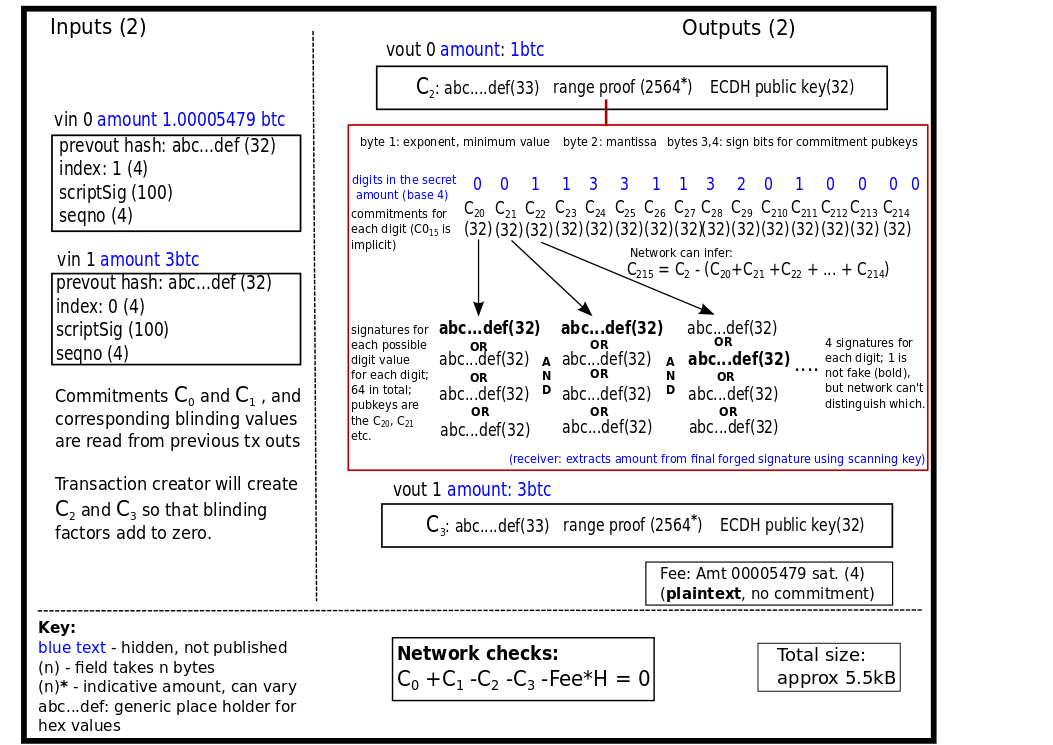
\includegraphics[scale=0.5]{transaction.png}
\caption{\emph{A near complete schematic of a CT transaction with 2 inputs and 2 outputs. The arrows show the path of serialization as it is published on the network. Some minor details are missing.}}
\end{figure}

\pagebreak

\subsection{Code references}
Most of the code for Confidential Transactions can be found in

\begin{verbatim}
src/secp256k1/src/{rangeproof_impl.h,borromean_impl.h}
and
src/{transaction.cpp, blind.cpp}
\end{verbatim}


\pagebreak

 \begin{thebibliography}{33}

  \bibitem{ct_wu} G. Maxwell, Confidential Transasctions write up \url{https://people.xiph.org/~greg/confidential_values.txt}
  \bibitem{chaum_bs} D. Chaum, Blind Signatures for Payments \url{http://www.hit.bme.hu/~buttyan/courses/BMEVIHIM219/2009/Chaum.BlindSigForPayment.1982.PDF}
  \bibitem{chaum_dc} D. Chaum, The Dining Cryptographers Problem: Unconditional Sender and Recipient Untraceability \url{http://www.cs.elte.hu/~rfid/dcrypt_chaum.html}
  \bibitem{ms_ringsig} How To Leak A Secret \url{https://research.microsoft.com/en-us/um/people/yael/publications/2006-leak_secret.pdf}
  \bibitem{borromean} G Maxwell, A Poelstra, Borromean Ring Signatures \url{https://github.com/Blockstream/borromean_paper/}
  \bibitem{pbtc} V Buterin, pybitcointools - one of a few similar libraries for working with Bitcoin operations in Python  \url{https://github.com/vbuterin/pybitcointools}
  \bibitem{rfc6979} RFC6979 Deterministic usage of the Digital Signature Algorithm: \url{https://tools.ietf.org/html/rfc6979}
  \bibitem{hmac} Wikipedia's description of HMAC: \url{https://en.wikipedia.org/wiki/Hash-based_message_authentication_code}
  \bibitem{secp256k1_nums} A discussion of the NUMS status of the secp256k1 curve (whole thread may be of interest) \url{https://bitcointalk.org/index.php?topic=289795.msg3204734#msg3204734}
  \bibitem{dhke} Wikipedia's description of Diffie Hellman key exchange: \url{https://en.wikipedia.org/wiki/Diffie%E2%80%93Hellman_key_exchange}
  \bibitem{residue} How to calculate y given x on the secp256k1 curve: \url{https://en.wikipedia.org/wiki/Quadratic_residue#Prime_or_prime_power_modulus}
  \bibitem{b58check} Base58check encoding description: \url{https://en.bitcoin.it/wiki/Base58Check_encoding}
  \bibitem{pedersen} T Pedersen, Original description of the concept behind Pedersen commitments - Non-Interactive and Information-Theoretic Secure Verifiable Secret Sharing  \url{http://link.springer.com/chapter/10.1007%2F3-540-46766-1_9}
  \bibitem{borring} A Gibson, An implementation of Borromean ring signatures in Python, for learning \url{https://github.com/AdamISZ/borring}
  \end{thebibliography}

\end{document}
